% ARTICLE ----
% This is just here so I know exactly what I'm looking at in Rstudio when messing with stuff.
\documentclass[11pt,]{article}
\usepackage[left=1in,top=1in,right=1in,bottom=1in]{geometry}
\newcommand*{\authorfont}{\fontfamily{phv}\selectfont}
\usepackage[]{libertine}


  \usepackage[T1]{fontenc}
  \usepackage[utf8]{inputenc}




\usepackage{abstract}
\renewcommand{\abstractname}{}    % clear the title
\renewcommand{\absnamepos}{empty} % originally center

\renewenvironment{abstract}
 {{%
    \setlength{\leftmargin}{0mm}
    \setlength{\rightmargin}{\leftmargin}%
  }%
  \relax}
 {\endlist}

\makeatletter
\def\@maketitle{%
 \newpage
%  \null
%  \vskip 2em%
%  \begin{center}%
{\fontsize{12}{12}\selectfont\raggedright \color{um-red}  This document is the preprint of the article published in Methods in Ecology and Evolution, DOI: 10.1111/2041-210X.14119 \vskip 13.5pt} 
  \let \footnote \thanks
    {\fontsize{18}{20}\selectfont\raggedright  \setlength{\parindent}{0pt} \@title \par}%
}
%\fi
\makeatother




\setcounter{secnumdepth}{0}


\usepackage{graphicx,grffile}
\makeatletter
\def\maxwidth{\ifdim\Gin@nat@width>\linewidth\linewidth\else\Gin@nat@width\fi}
\def\maxheight{\ifdim\Gin@nat@height>\textheight\textheight\else\Gin@nat@height\fi}
\makeatother
% Scale images if necessary, so that they will not overflow the page
% margins by default, and it is still possible to overwrite the defaults
% using explicit options in \includegraphics[width, height, ...]{}
\setkeys{Gin}{width=\maxwidth,height=\maxheight,keepaspectratio}


\title{Contrasted hindcast performances demonstrates the need for more
realistic models  }



\author{\Large Victor Van der Meersch
\footnote{Corresponding author - victor.vandermeersch@cefe.cnrs.fr}\vspace{0.05in} \newline\newline\normalsize\emph{CEFE,
Université de Montpellier, CNRS, EPHE, IRD, Montpellier,
France}   \and \Large Edward
Armstrong\vspace{0.05in} \newline\newline\normalsize\emph{Department of
Geosciences and Geography, University of Helsinki, Helsinki,
Finland}   \and \Large Florent
Mouillot\vspace{0.05in} \newline\newline\normalsize\emph{CEFE,
Université de Montpellier, CNRS, EPHE, IRD, Montpellier,
France}   \and \Large Frédérik
Saltré\vspace{0.05in} \newline\newline\normalsize\emph{Global Ecology
\textbar{} Partuyarta Ngadluku Wardli Kuu, College of Science and
Engineering, Flinders University, Adelaide,
Australia}   \and \Large Anne
Duputié\vspace{0.05in} \newline\newline\normalsize\emph{Université de
Lille, Sciences et Technologies, CNRS, UMR 8198-EEP-Evo-Eco-Pal?o,
Lille, France}   \and \Large Christophe
Randin\vspace{0.05in} \newline\newline\normalsize\emph{Univ. Lausanne,
Dept. of Ecology \& Evolution / Interdisciplinary Centre for Mountain
Research (CIRM), Biophore, Lausanne, Switzerland}   \and \Large Hendrik
Davi\vspace{0.05in} \newline\newline\normalsize\emph{INRAE, URFM,
Avignon, France}   \and \Large Isabelle
Chuine\vspace{0.05in} \newline\newline\normalsize\emph{CEFE, Université
de Montpellier, CNRS, EPHE, IRD, Montpellier, France}  }


\date{}

\usepackage{titlesec}

\titleformat*{\section}{\normalsize\bfseries}
\titleformat*{\subsection}{\normalsize\itshape}
\titleformat*{\subsubsection}{\normalsize\itshape}
\titleformat*{\paragraph}{\normalsize\itshape}
\titleformat*{\subparagraph}{\normalsize\itshape}



\usepackage{biblatex}

\addbibresource{bib/robustness\_bibliography.bib}


\newtheorem{hypothesis}{Hypothesis}
\usepackage{setspace}


% set default figure placement to htbp
\makeatletter
\def\fps@figure{htbp}
\makeatother

\usepackage{graphicx}
\usepackage{xcolor}
\usepackage{float}
\floatplacement{figure}{H}
\usepackage[width=.9\textwidth, font=small]{caption}
\usepackage{libertine}
\usepackage[left]{lineno}
\linenumbers
\renewcommand*{\thefootnote}{\fnsymbol{footnote}}

% move the hyperref stuff down here, after header-includes, to allow for - \usepackage{hyperref}

\makeatletter

\makeatother


% Add an option for endnotes. -----


% add tightlist ----------
\providecommand{\tightlist}{%
\setlength{\itemsep}{0pt}\setlength{\parskip}{0pt}}

% add some other packages ----------

% \usepackage{multicol}
% This should regulate where figures float
% See: https://tex.stackexchange.com/questions/2275/keeping-tables-figures-close-to-where-they-are-mentioned
\usepackage[section]{placeins}

% CSL environment change -----

\newlength{\cslhangindent}
\setlength{\cslhangindent}{1.5em}
\newlength{\csllabelwidth}
\setlength{\csllabelwidth}{3em}
\newenvironment{CSLReferences}[2] % #1 hanging-ident, #2 entry spacing
 {% don't indent paragraphs
  \setlength{\parindent}{0pt}
  % turn on hanging indent if param 1 is 1
  \ifodd #1 \everypar{\setlength{\hangindent}{\cslhangindent}}\ignorespaces\fi
  % set entry spacing
  \ifnum #2 > 0
  \setlength{\parskip}{#2\baselineskip}
  \fi
 }%
 {}
\usepackage{calc}
\newcommand{\CSLBlock}[1]{#1\hfill\break}
\newcommand{\CSLLeftMargin}[1]{\parbox[t]{\csllabelwidth}{#1}}
\newcommand{\CSLRightInline}[1]{\parbox[t]{\linewidth - \csllabelwidth}{#1}\break}
\newcommand{\CSLIndent}[1]{\hspace{\cslhangindent}#1}

% Last minute stuff -----
% \usepackage{amssymb,amsmath} % HT @ashenkin


% Add by VV
% \usepackage[dvipsnames]{xcolor} % clash with kableExtra ?
\PassOptionsToPackage{hyphens}{url} % url is loaded by hyperref
\usepackage[unicode=true]{hyperref}
  \PassOptionsToPackage{usenames,dvipsnames}{color} % color is loaded by hyperref
\definecolor{um-red}{RGB}{233,78,82}
\definecolor{um-gray}{RGB}{114,146,162}
\definecolor{blue-sapphire}{RGB}{0, 110, 144}
\hypersetup{
    colorlinks=true,
    linkcolor=um-red,
    citecolor=um-red,
    urlcolor=um-gray,
    breaklinks=true}
\urlstyle{same} % don't use monospace font for urls
\usepackage[capitalise, nameinlink]{cleveref}




\begin{document}

% \pagenumbering{arabic}% resets `page` counter to 1
%

% \maketitle



{% \usefont{T1}{pnc}{m}{n}
\setlength{\parindent}{0pt}
\thispagestyle{plain}
{\fontsize{18}{20}\selectfont\raggedright
\maketitle  % title \par

}



{
   \vskip 13.5pt\relax \normalsize\fontsize{11}{12}
\textbf{\authorfont Victor Van der Meersch
\footnote{Corresponding author - victor.vandermeersch@cefe.cnrs.fr}} \hskip 15pt \emph{\small CEFE,
Université de Montpellier, CNRS, EPHE, IRD, Montpellier,
France}   \par \textbf{\authorfont Edward
Armstrong} \hskip 15pt \emph{\small Department of Geosciences and
Geography, University of Helsinki, Helsinki,
Finland}   \par \textbf{\authorfont Florent
Mouillot} \hskip 15pt \emph{\small CEFE, Université de Montpellier,
CNRS, EPHE, IRD, Montpellier,
France}   \par \textbf{\authorfont Frédérik
Saltré} \hskip 15pt \emph{\small Global Ecology \textbar{} Partuyarta
Ngadluku Wardli Kuu, College of Science and Engineering, Flinders
University, Adelaide, Australia}   \par \textbf{\authorfont Anne
Duputié} \hskip 15pt \emph{\small Université de Lille, Sciences et
Technologies, CNRS, UMR 8198-EEP-Evo-Eco-Pal?o, Lille,
France}   \par \textbf{\authorfont Christophe
Randin} \hskip 15pt \emph{\small Univ. Lausanne, Dept. of Ecology \&
Evolution / Interdisciplinary Centre for Mountain Research (CIRM),
Biophore, Lausanne, Switzerland}   \par \textbf{\authorfont Hendrik
Davi} \hskip 15pt \emph{\small INRAE, URFM, Avignon,
France}   \par \textbf{\authorfont Isabelle
Chuine} \hskip 15pt \emph{\small CEFE, Université de Montpellier, CNRS,
EPHE, IRD, Montpellier, France}   

}

}








\begin{abstract}

    \hbox{\vrule height .2pt width 39.14pc}

    \vskip 8.5pt % \small

\noindent While process-based models are expected to provide better
species range shift predictions under novel environmental conditions
than correlative counterparts, this hypothesis has yet to be tested.

We used both process- and correlative-based species distribution models
to hindcast the range shift of 5 tree species across Europe for the last
15,000 years and evaluated these outputs against fossil pollen records.
Using these results and considering the expected magnitude of climate
novelty, we then quantified model uncertainties under future climate
scenarios.

We show that long-term hindcast decreases overall model performances and
even the most promising approach (process-based models calibrated using
occurrence data) is unlikely to provide any reliable projections under
future no-analog conditions.

Our results (i) challenge the concept of transferability in species
distribution modelling, (ii) highlight the prerequisites for ensuring
model robustness and (iii) provide a promising framework to scale up
complex models and promote their use in an ever-changing world.


\vskip 8.5pt \noindent \emph{Keywords}: keyword1, keyword2 \par

    \hbox{\vrule height .2pt width 39.14pc}



\end{abstract}


\vskip -8.5pt


 % removetitleabstract

\noindent \doublespacing

\hypertarget{introduction}{%
\section{Introduction}\label{introduction}}

Model simulations are a fundamental source for improving our
understanding of past, present and future climate impacts on ecosystems
and species distribution -- provided that we can trust them. As the
demand for reliable projections is increasing, the systematic evaluation
of model skill should be one of the main concerns of modellers. Such
evaluation remains critical to build confidence in our models, and plays
a crucial role in providing the most credible information on the impacts
of climate change so that stakeholders can make informed decisions
(\protect\hyperlink{ref-Dawson2011}{Dawson \emph{et al.} 2011};
\protect\hyperlink{ref-Mouquet2015}{Mouquet \emph{et al.} 2015}).

The unforeseen will always remain so, and the accuracy of model future
projections cannot thus be tested directly. Therefore, the most
straightforward approach to evaluate models is to compare their output
with what we know from the past. Plausibly reproducing the past
(hindcast performance/skill) can be seen as a requisite condition to be
considered a viable model for future projections (forecast reliability).
Even if there is no observed period with climate conditions exactly
matching those expected over the 21st century
(\protect\hyperlink{ref-Burke2018}{Burke \emph{et al.} 2018}),
hindcasting exercises can still increase our confidence that the models
represent, implicitly or explicitly, the essential processes for the
simulation of future species range shifts.

In this regard, recent past observations (typically for a few decades)
have been used for testing SDM predictions over time (e.g.
\protect\hyperlink{ref-Araujo2005}{Araújo \emph{et al.} 2005};
\protect\hyperlink{ref-Kharouba2009}{Kharouba \emph{et al.} 2009};
\protect\hyperlink{ref-Smith2013}{Smith \emph{et al.} 2013}).
{[}Résultats de ces études ?{]}. However, as they were made in a limited
climate range similar to calibration conditions, they do not enable
fully independent model evaluation. By looking much further back in the
past, paleoenvironments offer a unique framework to test species
distribution model transferability in more challenging conditions, in
the same way as climate models are evaluated using palaeodata
(\protect\hyperlink{ref-Braconnot2012}{Braconnot \emph{et al.} 2012}).
Simulations in distant past (spanning several millennia) allow for model
evaluation under conditions significantly different from present-day
(\protect\hyperlink{ref-Maguire2015}{Maguire \emph{et al.} 2015}), where
climate variations were larger than those encountered during the last
century. Taking advantage of the available paleo-archives is a great
opportunity to understand long-term climate-biodiversity dynamics
(\protect\hyperlink{ref-Fordham2020}{Fordham \emph{et al.} 2020}).
Several studies have tested the transferability of species distribution
models using paleoclimate reconstructions and fossil records (e.g.
\protect\hyperlink{ref-Pearman2008}{Pearman \emph{et al.} 2008};
\protect\hyperlink{ref-Veloz2012}{Veloz \emph{et al.} 2012};
\protect\hyperlink{ref-Williams2013}{Williams \emph{et al.} 2013}). They
all show a decrease of the ability of SDMs to simulate past species
distributions. Their findings remind us to exercise caution when
interpreting their projections in novel climates that differ
significantly from the present
(\protect\hyperlink{ref-Maguire2016}{Maguire \emph{et al.} 2016}),
especially as no-analogues climate conditions are forecasted to become
common (\protect\hyperlink{ref-Williams2007}{Williams \emph{et al.}
2007}) and may compromised the accuracy of model predictions
(\protect\hyperlink{ref-Fitzpatrick2018}{Fitzpatrick \emph{et al.}
2018}). These investigations have yielded valuable insights into the
reliability of species distribution models, but have primarily focused
on correlative models, despite the growing interest of process-based
models in predictive ecology (\protect\hyperlink{ref-Urban2016}{Urban
\emph{et al.} 2016}; \protect\hyperlink{ref-Connolly2017}{Connolly
\emph{et al.} 2017}; \protect\hyperlink{ref-Pilowsky2022}{Pilowsky
\emph{et al.} 2022}).

This omission represents a notable gap in our understanding of the
tenets of species distribution modelling, as only one side of the
continuum between statistical and mechanistic approaches has been
explored (\protect\hyperlink{ref-Dormann2012}{Dormann \emph{et al.}
2012}), neglecting the investigation of process-based model performance.
Rather than inferring correlations between observations and potential
environmental drivers, these models are built upon explicit causal
relationships determined experimentally representing physiological,
ecological and demographic processes. Their projections in response to
climate change differ from correlative models, the latter being
systematically more pessimistic {[}références{]}. However, very few
studies have gone beyond these qualitative comparisons and really
examined how they are performing, with virtual species
(\protect\hyperlink{ref-Zurell2016}{Zurell \emph{et al.} 2016}), exotic
species in new colonized areas
(\protect\hyperlink{ref-Higgins2020}{Higgins \emph{et al.} 2020}), or in
the recent past (\protect\hyperlink{ref-Fordham2018}{Fordham \emph{et
al.} 2018}). Therefore, despite process-based models have shown their
usefulness for paleoecological studies {[}références{]}, the extent to
which the potential benefits of process-based models translate into
improved predictions in really different climatic conditions remains
unknown \protect\hyperlink{ref-Briscoe2019}{Briscoe \emph{et al.}}
(\protect\hyperlink{ref-Briscoe2019}{2019}). Addressing this gap by a
thorough evaluation of the different class of models is crucial
(\protect\hyperlink{ref-Evans2016}{Evans \emph{et al.} 2016}), as
process-based models hold the potential to enhance our ability to
predict species responses to climate change and to provide more robust
projections in novel conditions (\protect\hyperlink{ref-Evans2012}{Evans
2012}; \protect\hyperlink{ref-Singer2016}{Singer \emph{et al.} 2016}).

Here, we propose a state-of-the-art comparison of the skills of
correlative models and process-based models to simulate the
paleodistributions of emblematic tree species of Europe. In order to
fully explore the different classes of models, we use different versions
of the models that differ by their level of complexity and the methods
of estimation of their parameters. In particular, as hybrid models
(sensu \protect\hyperlink{ref-Dormann2012}{Dormann \emph{et al.} 2012})
have been raised as a potential avenue by borrowing strength from both
statistical and process-based approaches
(\protect\hyperlink{ref-Evans2016}{Evans \emph{et al.} 2016}), we use
inverse modelling to fit the process-based models in the same way as the
correlative models (\protect\hyperlink{ref-VanderMeersch2023}{Van der
Meersch \& Chuine 2023}). By encompassing the entire spectrum of models,
from correlative models to process-based models and their hybrid
data-driven counterparts, our comprehensive approach allows us to gain a
holistic understanding of the key features necessary for building
reliable models.

\begin{figure}
\centering
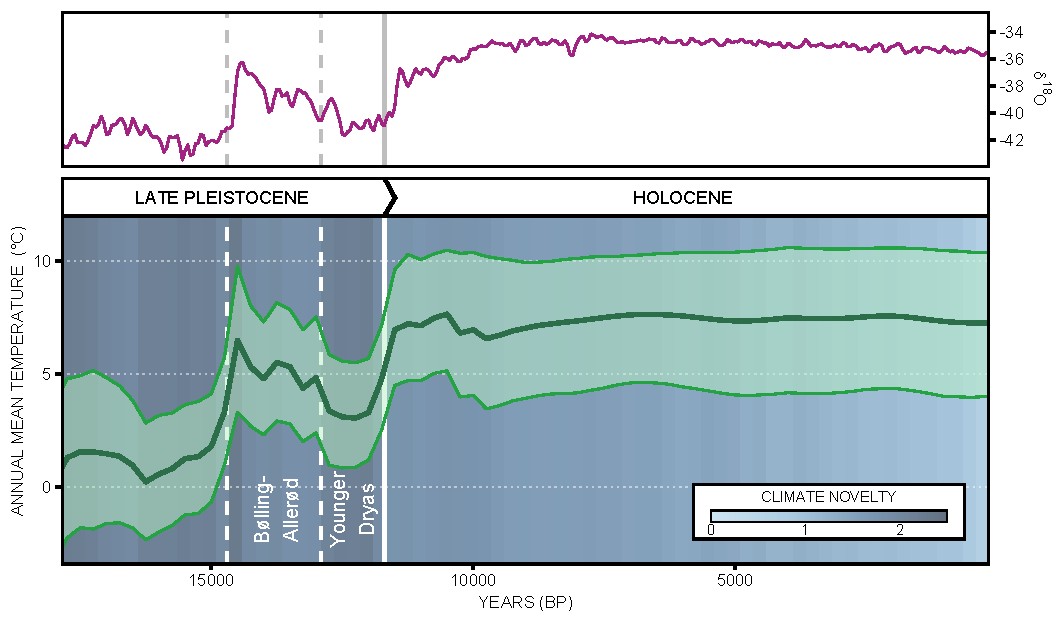
\includegraphics{paper_files/figure-latex/figure_climate_overview-1.pdf}
\caption{Climate overview}
\end{figure}

\begin{figure}
\centering
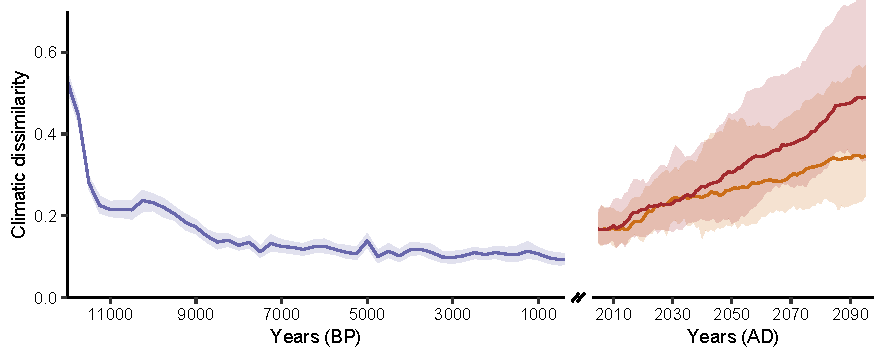
\includegraphics{paper_files/figure-latex/figure_climatedissimilarity-1.pdf}
\caption{Climate overview}
\end{figure}

\begin{figure}
\centering
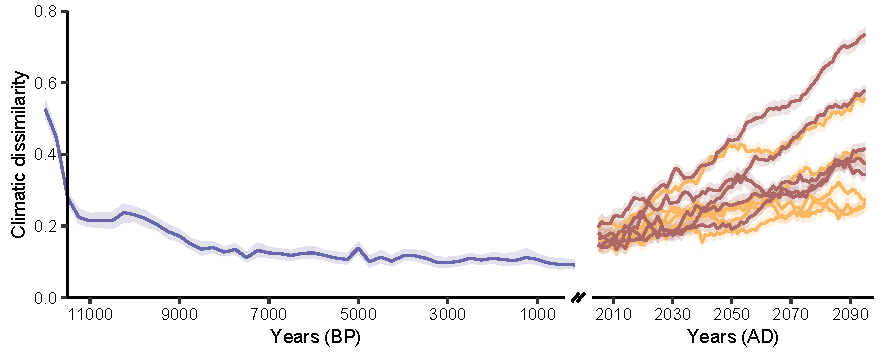
\includegraphics{paper_files/figure-latex/figure_climatedissimilaritybis-1.pdf}
\caption{Climate overview}
\end{figure}

\begin{figure}
\centering
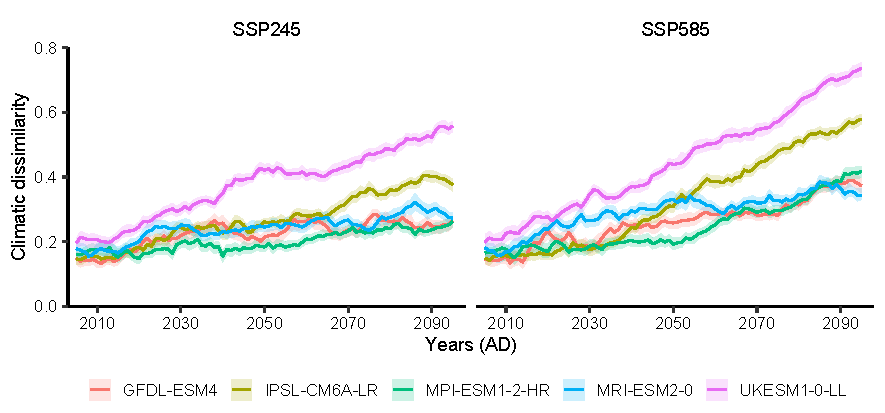
\includegraphics{paper_files/figure-latex/figure_climatedissimilarityGCM-1.pdf}
\caption{Climate overview}
\end{figure}

\hypertarget{results}{%
\section{Results}\label{results}}

\begin{figure}
\centering
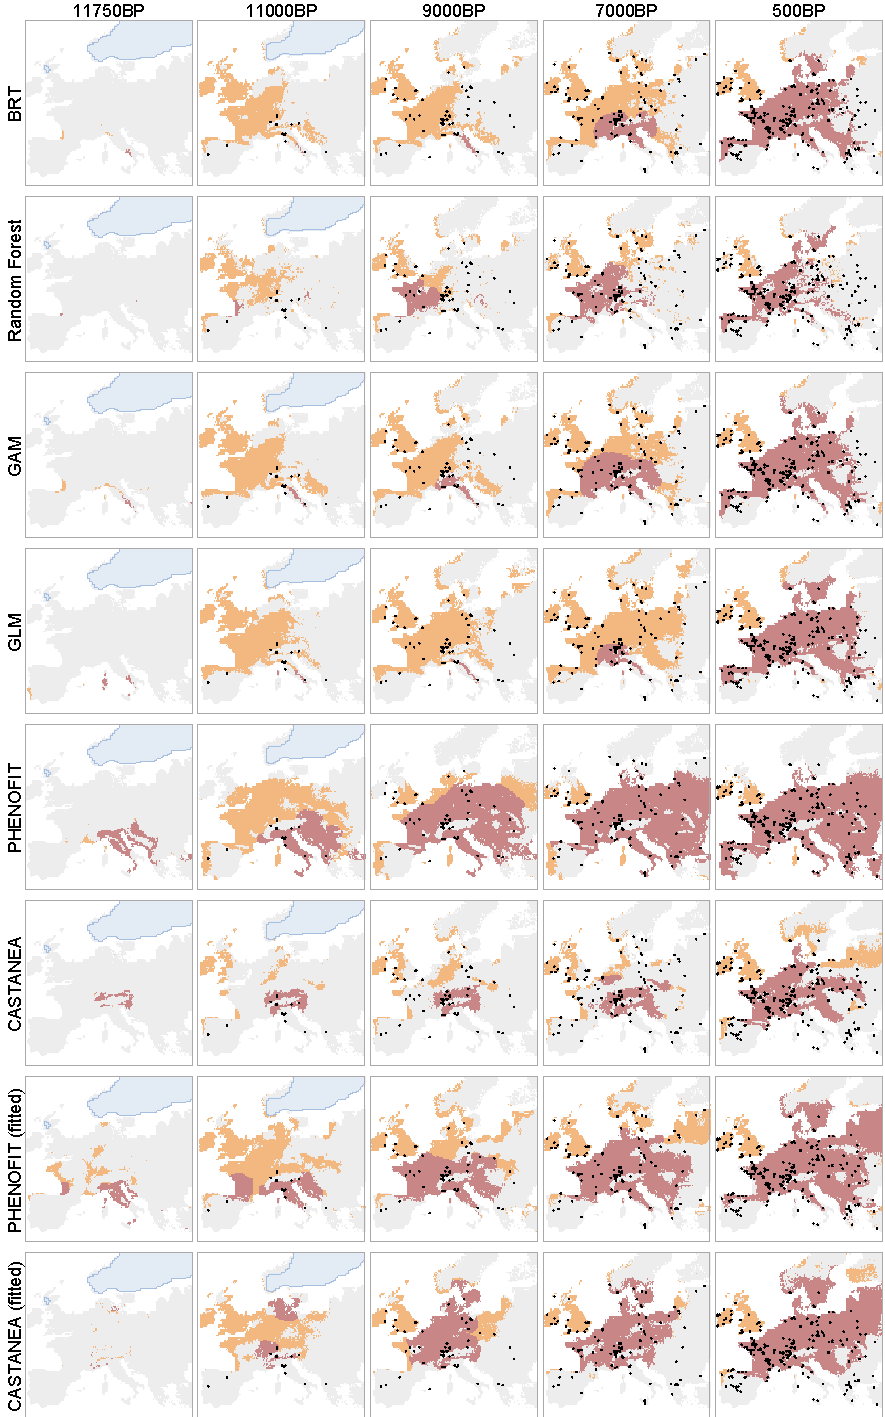
\includegraphics{paper_files/figure-latex/figure_2-1.pdf}
\caption{Sorensen Index, ordered Beta regression}
\end{figure}

\begin{verbatim}
## 
## alpha = 0.05
## Reject Ho if p <= alpha/2
## 
## alpha = 0.05
## Reject Ho if p <= alpha/2
\end{verbatim}

\begin{verbatim}
## 
## alpha = 0.05
## Reject Ho if p <= alpha/2
## 
## alpha = 0.05
## Reject Ho if p <= alpha/2
\end{verbatim}

\begin{verbatim}
## 
## alpha = 0.05
## Reject Ho if p <= alpha/2
\end{verbatim}

\begin{figure}
\centering
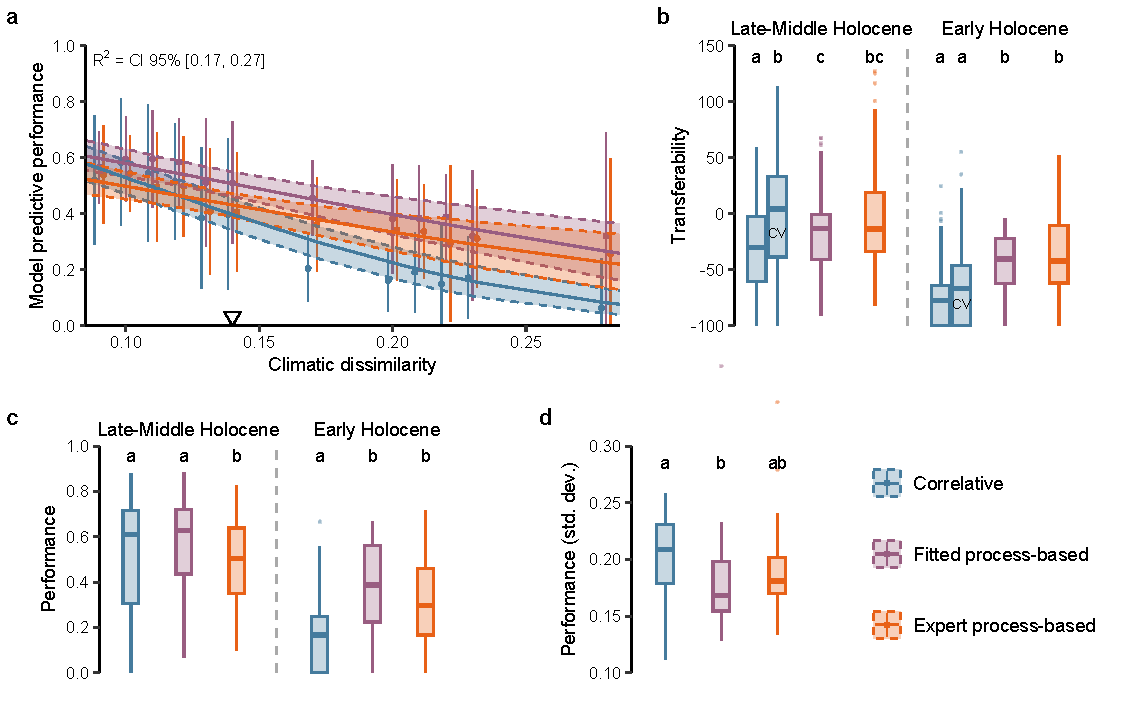
\includegraphics{paper_files/figure-latex/figure_3bis-1.pdf}
\caption{Sorensen Index, ordered Beta regression}
\end{figure}

\hypertarget{discussion}{%
\section{Discussion}\label{discussion}}

\hypertarget{methods}{%
\section{Methods}\label{methods}}

\hypertarget{late-quaternary-climate-and-vegetation}{%
\subsection{1. Late Quaternary climate and
vegetation}\label{late-quaternary-climate-and-vegetation}}

We used a monthly paleoclimate reconstruction dataset
(\protect\hyperlink{ref-Armstrong2019}{Armstrong \emph{et al.} 2019}),
generated with the HadCM3B-M2.1 coupled general circulation model, from
18.000BP. It includes both millennial scale climate variability and
inter-annual variability. For this work, several variables were
specifically produced: mean temperature, average minimum and maximum
daily temperatures, precipitation, number of rainy days, cloudiness, and
wind speed. We further downscaled temperature and precipitation monthly
data to 0.25° resolution, by applying a height correction of
coarse-scale variables towards an elevation level at high resolution
(from the ICE-6G\_C dataset, \protect\hyperlink{ref-Peltier2015}{Peltier
\emph{et al.} 2015}).\\
We then generated daily data (temperatures, precipitation, cloud cover
and wind speed) using the weather generator GWGEN
(\protect\hyperlink{ref-Sommer2017}{Sommer \& Kaplan 2017}), for 30-year
period every 250 years. We simulated daily extra-terrestrial solar
radiation (with the same orbital forcing conditions used by
\protect\hyperlink{ref-Armstrong2019}{Armstrong \emph{et al.} 2019}) and
then computed daily global radiation using previously generated daily
cloud-cover data (as implemented in LPJ-LMfire global model,
\protect\hyperlink{ref-Pfeiffer2013}{Pfeiffer \emph{et al.} 2013}).
Finally, we computed potential evapotranspiration following the standard
FAO Penman-Monteith method.

Fossil pollen records were extracted from the LegacyPollen dataset
(\protect\hyperlink{ref-Herzschuh2022}{Herzschuh \emph{et al.} 2022}).
This dataset is mainly based on the Neotoma database
(\protect\hyperlink{ref-Williams2018}{Williams \emph{et al.} 2018}), and
provides samples with standardized chronologies and age uncertainties.
We removed sites that had marine depositional environments
(\protect\hyperlink{ref-Maguire2016}{Maguire \emph{et al.} 2016}), and
only kept samples with more than 200 pollen grain counts and age
uncertainty of less than 500 years. Pollen relative abundances were
interpolated to consecutive 500-year intervals. If multiple samples from
the same site belonged to the same period, we averaged their pollen
abundances, weighting by their age uncertainty and temporal distance
from the center of the period. Relative genus pollen abundances were
converted to presence/absence using thresholds of 1\% for \emph{Fagus}
and \emph{Abies}, and 2.5\% for \emph{Quercus} (based on biome
reconstructions, \protect\hyperlink{ref-Williams1998}{Williams \emph{et
al.} 1998}). If several sites fell within the same grid cell (0.25°), we
considered the species as present if there was at least one record.

\hypertarget{species-distribution-modeling}{%
\subsection{2. Species distribution
modeling}\label{species-distribution-modeling}}

Two process-based models were used in this study. PHENOFIT focuses on
phenology and how it relates to survival and reproduction
(\protect\hyperlink{ref-Chuine2001}{Chuine \& Beaubien 2001}), and has
been validated for several North American and European species (e.g.
\protect\hyperlink{ref-Morin2007}{Morin \emph{et al.} 2007};
\protect\hyperlink{ref-Saltre2013}{Saltré \emph{et al.} 2013};
\protect\hyperlink{ref-Duputie2015}{Duputié \emph{et al.} 2015};
\protect\hyperlink{ref-Gauzere2020}{Gauzere \emph{et al.} 2020}).
CASTANEA is much more complex, and focuses on carbon and water cycles
(\protect\hyperlink{ref-Dufrene2005}{Dufrêne \emph{et al.} 2005}). It
was successfully applied to several European species (e.g.
\protect\hyperlink{ref-Davi2006}{Davi \emph{et al.} 2006};
\protect\hyperlink{ref-Delpierre2012}{Delpierre \emph{et al.} 2012};
\protect\hyperlink{ref-Davi2017}{Davi \& Cailleret 2017}).\\
For both models, two versions were employed: one is calibrated with
expert knowledge, observations and measurements of the processes
modelled (expert calibration), and the other is calibrated using species
distribution data (inverse calibration,
\protect\hyperlink{ref-VanderMeersch2023}{Van der Meersch \& Chuine
2023}).

Four well-established correlative models, whose predictive performances
have been tested (\protect\hyperlink{ref-Valavi2022}{Valavi \emph{et
al.} 2022}), were implemented: GLM with lasso regularization, GAM, BRT
and down-sampled Random Forest. We chose four uncorrelated climate
predictors related to ecological processes: minimum temperature of the
coldest month (frost tolerance), total precipitation (accumulated
water), GDD (\textgreater5°C) between April and September (vegetation
growth and fruit maturation), water balance between June and July
(summer drought). We also included two soil covariates (pH and WHC). For
each statistical model and each species, we run a fivefold environmental
cross-validation to check model performance. We then use all the
available training data to calibrate the models, in order to favour
final prediction quality (\protect\hyperlink{ref-Roberts2017}{Roberts
\emph{et al.} 2017}).

Model calibrations (both for correlative and inverse-calibrated
process-based model) were performed in the historical climate
(1970-2000), extracted from ERA5-Land hourly dataset
(\protect\hyperlink{ref-Sabater2019}{\textbf{Sabater2019?}};
\protect\hyperlink{ref-Sabater2021}{\textbf{Sabater2021?}}). The species
occurrence data we used for model fitting came from the dataset
assembled in \protect\hyperlink{ref-VanderMeersch2023}{Van der Meersch
\& Chuine} (\protect\hyperlink{ref-VanderMeersch2023}{2023}).

Paleosimulations were runned for 30-year period every 250 years, for
five species: \emph{Fagus sylvatica}, \emph{Abies alba}, \emph{Quercus
robur}, \emph{Quercus petraea} and \emph{Quercus ilex}. Model outputs
were averaged over each 30-year period.

\hypertarget{tree-migration}{%
\subsection{3. Tree migration}\label{tree-migration}}

Neglecting tree migration in an hindcasting experiment can lead to
misleading predictions. To implement these dispersal constraints, we run
a simple cellular automaton (\protect\hyperlink{ref-Engler2012}{Engler
\emph{et al.} 2012}), assuming that trees can disperse once a year. We
modified the initial version of this dispersal model in order to use
both short- and long-distance dispersal kernels. We used
species-specific fat-tailed kernels (calibrated in
\protect\hyperlink{ref-Zani2022}{Zani \emph{et al.} 2022}), at a 500m
resolution. Model outputs were classified in two classes, using specific
optimal thresholds (Youden index-based cut-off points) which maximize
model performance in the historical climate: (i) cells where the species
cannot survived (under the threshold) were assigned a zero fitness, and
(ii) cells where the species can migrate (above the threshold), for
which the fitness was rescaled between 0 and 1.\\
\emph{Fagus} and \emph{Abies} migration simulations started from
12.000BP, while \emph{Quercus} simulations started from 15.000BP (to
take into account the potential spread of \emph{Quercus} during the
Lateglacial period). We considered \emph{Fagus sylvatica} and
\emph{Abies alba} as the major representatives of their genus. For
\emph{Quercus} species, we runned two separate migration simulations for
deciduous and evergreen individuals, that we then assembled. We
considered the \emph{Quercus} deciduous fitness as the maximum fitness
between \emph{Q. robur} and \emph{Q. petraea}.\\
Migration starting points (refugia) were assessed by complementing
LegacyPollen data with other sources, such as macrofossils
(\protect\hyperlink{ref-TerhuerneBerson2004}{Terhürne-Berson \emph{et
al.} 2004}; \protect\hyperlink{ref-Magri2006}{Magri \emph{et al.} 2006};
\protect\hyperlink{ref-Tzedakis2013}{Tzedakis \emph{et al.} 2013}).
These complementary points were not used for model performance
evaluation afterwards.

\hypertarget{model-skill-in-past-and-future-environments}{%
\subsection{4. Model skill in past and future
environments}\label{model-skill-in-past-and-future-environments}}

We used the True Skill Statistic (TSS) to measure the hindcast skill of
our models, based on the confusion matrix. We compared the area
colonized after the migration simulations to the presence/absence data
extracted from the LegacyPollen dataset, at each 500-year interval.

In order to quantify the novel conditions under which models were
projected, we computed climate dissimilarity as the minimum Mahalanobis
distance (which accounts for covariance among variables), with vectors
of three-month means temperature and three-month sums of precipitation
(\protect\hyperlink{ref-Burke2019}{Burke \emph{et al.} 2019}), between
each cell of the projected period and all the cells of the baseline
climate (the CRU TS v. 4.07 gridded dataset,
\protect\hyperlink{ref-Harris2020}{Harris \emph{et al.} 2020}).\\
We computed this climatic metric for past conditions and for future
conditions (5 climate models and 2 scenarios from the CMIP6 experiment,
\protect\hyperlink{ref-Noel2020}{\textbf{Noel2020?}}). Both paleoclimate
and future climate data were uniformized with CRU dataset to maximize
comparability among paleoclimate and future climate novelties. The
difference (for three-month temperature average) and the ratio (for
three-month precipitation sum) between the observations (from 1921 to
1980) and simulations (1921-1950 for HadCM3B, 1951-1980 for CMIP6
projections) were calculated and applied to the whole modeled time
period, assuming that the bias was constant.

Finally, we fitted linear-plateau regressions, which follow two phases
(a flat plateau and a linear response), between median realized model
skill and past climate novelty. These regressions allow us to compute
tipping points, above which model predictive ability decreases strongly.
The confidence intervals were calculated with the R package
\emph{propagate} (\protect\hyperlink{ref-Spiess2018}{Spiess 2018}), by
using first and second-order Taylor expansion and Monte Carlo
simulations. To check whether our approach was not too deterministic, we
also fitted generalized additive models which gave the same patterns
(Supplementary Figure).

\hypertarget{supplementary-material}{%
\section{Supplementary material}\label{supplementary-material}}

\hypertarget{references}{%
\section{References}\label{references}}

\setlength{\parindent}{-0.2in}
\setlength{\leftskip}{0.2in}
\setlength{\parskip}{8pt}
\vspace*{-0.2in}

\noindent

\hypertarget{refs}{}
\begin{CSLReferences}{1}{0}
\leavevmode\vadjust pre{\hypertarget{ref-Araujo2005}{}}%
Araújo, M.B., Pearson, R.G., Thuiller, W. \& Erhard, M. (2005).
Validation of species--climate impact models under climate change.
\emph{Global Change Biology}, \textbf{11}, 1504--1513.
\href{https://doi.org/10.1111/j.1365-2486.2005.01000.x}{10.1111/j.1365-2486.2005.01000.x}

\leavevmode\vadjust pre{\hypertarget{ref-Armstrong2019}{}}%
Armstrong, E., Hopcroft, P.O. \& Valdes, P.J. (2019). A simulated
{Northern} {Hemisphere} terrestrial climate dataset for the past 60,000
years. \emph{Scientific Data}, \textbf{6}, 265.
\href{https://doi.org/10.1038/s41597-019-0277-1}{10.1038/s41597-019-0277-1}

\leavevmode\vadjust pre{\hypertarget{ref-Braconnot2012}{}}%
Braconnot, P., Harrison, S.P., Kageyama, M., Bartlein, P.J.,
Masson-Delmotte, V., Abe-Ouchi, A., Otto-Bliesner, B. \& Zhao, Y.
(2012). Evaluation of climate models using palaeoclimatic data.
\emph{Nature Climate Change}, \textbf{2}, 417--424.
\href{https://doi.org/10.1038/nclimate1456}{10.1038/nclimate1456}

\leavevmode\vadjust pre{\hypertarget{ref-Briscoe2019}{}}%
Briscoe, N.J., Elith, J., Salguero-Gómez, R., Lahoz-Monfort, J.J.,
Camac, J.S., Giljohann, K.M., Holden, M.H., Hradsky, B.A., Kearney,
M.R., McMahon, S.M., Phillips, B.L., Regan, T.J., Rhodes, J.R., Vesk,
P.A., Wintle, B.A., Yen, J.D.L. \& Guillera-Arroita, G. (2019).
Forecasting species range dynamics with process-explicit models:
Matching methods to applications. \emph{Ecology Letters}, \textbf{22},
1940--1956. \href{https://doi.org/10.1111/ele.13348}{10.1111/ele.13348}

\leavevmode\vadjust pre{\hypertarget{ref-Burke2019}{}}%
Burke, K.D., Williams, J.W., Brewer, S., Finsinger, W., Giesecke, T.,
Lorenz, D.J. \& Ordonez, A. (2019). Differing climatic mechanisms
control transient and accumulated vegetation novelty in {Europe} and
eastern {North} {America}. \emph{Philosophical Transactions of the Royal
Society B: Biological Sciences}, \textbf{374}, 20190218.
\href{https://doi.org/10.1098/rstb.2019.0218}{10.1098/rstb.2019.0218}

\leavevmode\vadjust pre{\hypertarget{ref-Burke2018}{}}%
Burke, K.D., Williams, J.W., Chandler, M.A., Haywood, A.M., Lunt, D.J.
\& Otto-Bliesner, B.L. (2018). Pliocene and {Eocene} provide best
analogs for near-future climates. \emph{Proceedings of the National
Academy of Sciences}, \textbf{115}, 13288--13293.
\href{https://doi.org/10.1073/pnas.1809600115}{10.1073/pnas.1809600115}

\leavevmode\vadjust pre{\hypertarget{ref-Chuine2001}{}}%
Chuine, I. \& Beaubien, E.G. (2001). Phenology is a major determinant of
tree species range. \emph{Ecology Letters}, \textbf{4}, 500--510.
\href{https://doi.org/10.1046/j.1461-0248.2001.00261.x}{10.1046/j.1461-0248.2001.00261.x}

\leavevmode\vadjust pre{\hypertarget{ref-Connolly2017}{}}%
Connolly, S.R., Keith, S.A., Colwell, R.K. \& Rahbek, C. (2017).
Process, {Mechanism}, and {Modeling} in {Macroecology}. \emph{Trends in
Ecology \& Evolution}, \textbf{32}, 835--844.
\href{https://doi.org/10.1016/j.tree.2017.08.011}{10.1016/j.tree.2017.08.011}

\leavevmode\vadjust pre{\hypertarget{ref-Davi2017}{}}%
Davi, H. \& Cailleret, M. (2017). Assessing drought-driven mortality
trees with physiological process-based models. \emph{Agricultural and
Forest Meteorology}, \textbf{232}, 279--290.
\href{https://doi.org/10.1016/j.agrformet.2016.08.019}{10.1016/j.agrformet.2016.08.019}

\leavevmode\vadjust pre{\hypertarget{ref-Davi2006}{}}%
Davi, H., Dufrêne, E., Francois, C., Le Maire, G., Loustau, D., Bosc,
A., Rambal, S., Granier, A. \& Moors, E. (2006). Sensitivity of water
and carbon fluxes to climate changes from 1960 to 2100 in {European}
forest ecosystems. \emph{Agricultural and Forest Meteorology},
\textbf{141}, 35--56.
\href{https://doi.org/10.1016/j.agrformet.2006.09.003}{10.1016/j.agrformet.2006.09.003}

\leavevmode\vadjust pre{\hypertarget{ref-Dawson2011}{}}%
Dawson, T.P., Jackson, S.T., House, J.I., Prentice, I.C. \& Mace, G.M.
(2011). Beyond {Predictions}: {Biodiversity} {Conservation} in a
{Changing} {Climate}. \emph{Science}, \textbf{332}, 53--58.
\href{https://doi.org/10.1126/science.1200303}{10.1126/science.1200303}

\leavevmode\vadjust pre{\hypertarget{ref-Delpierre2012}{}}%
Delpierre, N., Soudani, K., François, C., Le Maire, G., Bernhofer, C.,
Kutsch, W., Misson, L., Rambal, S., Vesala, T. \& Dufrêne, E. (2012).
Quantifying the influence of climate and biological drivers on the
interannual variability of carbon exchanges in {European} forests
through process-based modelling. \emph{Agricultural and Forest
Meteorology}, \textbf{154-155}, 99--112.
\href{https://doi.org/10.1016/j.agrformet.2011.10.010}{10.1016/j.agrformet.2011.10.010}

\leavevmode\vadjust pre{\hypertarget{ref-Dormann2012}{}}%
Dormann, C.F., Schymanski, S.J., Cabral, J., Chuine, I., Graham, C.,
Hartig, F., Kearney, M., Morin, X., Römermann, C., Schröder, B. \&
Singer, A. (2012). Correlation and process in species distribution
models: Bridging a dichotomy. \emph{Journal of Biogeography},
\textbf{39}, 2119--2131.
\href{https://doi.org/10.1111/j.1365-2699.2011.02659.x}{10.1111/j.1365-2699.2011.02659.x}

\leavevmode\vadjust pre{\hypertarget{ref-Dufrene2005}{}}%
Dufrêne, E., Davi, H., François, C., Maire, G. le, Dantec, V.L. \&
Granier, A. (2005). Modelling carbon and water cycles in a beech forest:
{Part} {I}: {Model} description and uncertainty analysis on modelled
{NEE}. \emph{Ecological Modelling}, \textbf{185}, 407--436.
\href{https://doi.org/10.1016/j.ecolmodel.2005.01.004}{10.1016/j.ecolmodel.2005.01.004}

\leavevmode\vadjust pre{\hypertarget{ref-Duputie2015}{}}%
Duputié, A., Rutschmann, A., Ronce, O. \& Chuine, I. (2015).
Phenological plasticity will not help all species adapt to climate
change. \emph{Global Change Biology}, \textbf{21}, 3062--3073.
\href{https://doi.org/10.1111/gcb.12914}{10.1111/gcb.12914}

\leavevmode\vadjust pre{\hypertarget{ref-Engler2012}{}}%
Engler, R., Hordijk, W. \& Guisan, A. (2012). The {MIGCLIM} {R} package
-- seamless integration of dispersal constraints into projections of
species distribution models. \emph{Ecography}, \textbf{35}, 872--878.
\href{https://doi.org/10.1111/j.1600-0587.2012.07608.x}{10.1111/j.1600-0587.2012.07608.x}

\leavevmode\vadjust pre{\hypertarget{ref-Evans2012}{}}%
Evans, M.R. (2012). Modelling ecological systems in a changing world.
\emph{Philosophical Transactions of the Royal Society B: Biological
Sciences}, \textbf{367}, 181--190.
\href{https://doi.org/10.1098/rstb.2011.0172}{10.1098/rstb.2011.0172}

\leavevmode\vadjust pre{\hypertarget{ref-Evans2016}{}}%
Evans, M.E.K., Merow, C., Record, S., McMahon, S.M. \& Enquist, B.J.
(2016). Towards {Process}-based {Range} {Modeling} of {Many} {Species}.
\emph{Trends in Ecology \& Evolution}, \textbf{31}, 860--871.
\href{https://doi.org/10.1016/j.tree.2016.08.005}{10.1016/j.tree.2016.08.005}

\leavevmode\vadjust pre{\hypertarget{ref-Fitzpatrick2018}{}}%
Fitzpatrick, M.C., Blois, J.L., Williams, J.W., Nieto-Lugilde, D.,
Maguire, K.C. \& Lorenz, D.J. (2018). How will climate novelty influence
ecological forecasts? {Using} the {Quaternary} to assess future
reliability. \emph{Global Change Biology}, \textbf{24}, 3575--3586.
\href{https://doi.org/10.1111/gcb.14138}{10.1111/gcb.14138}

\leavevmode\vadjust pre{\hypertarget{ref-Fordham2018}{}}%
Fordham, D.A., Bertelsmeier, C., Brook, B.W., Early, R., Neto, D.,
Brown, S.C., Ollier, S. \& Araújo, M.B. (2018). How complex should
models be? {Comparing} correlative and mechanistic range dynamics
models. \emph{Global Change Biology}, \textbf{24}, 1357--1370.
\href{https://doi.org/10.1111/gcb.13935}{10.1111/gcb.13935}

\leavevmode\vadjust pre{\hypertarget{ref-Fordham2020}{}}%
Fordham, D.A., Jackson, S.T., Brown, S.C., Huntley, B., Brook, B.W.,
Dahl-Jensen, D., Gilbert, M.T.P., Otto-Bliesner, B.L., Svensson, A.,
Theodoridis, S., Wilmshurst, J.M., Buettel, J.C., Canteri, E., McDowell,
M., Orlando, L., Pilowsky, J.A., Rahbek, C. \& Nogues-Bravo, D. (2020).
Using paleo-archives to safeguard biodiversity under climate change.
\emph{Science}, \textbf{369}, eabc5654.
\href{https://doi.org/10.1126/science.abc5654}{10.1126/science.abc5654}

\leavevmode\vadjust pre{\hypertarget{ref-Gauzere2020}{}}%
Gauzere, J., Teuf, B., Davi, H., Chevin, L.-M., Caignard, T., Leys, B.,
Delzon, S., Ronce, O. \& Chuine, I. (2020). Where is the optimum?
{Predicting} the variation of selection along climatic gradients and the
adaptive value of plasticity. {A} case study on tree phenology.
\emph{Evolution Letters}, \textbf{4}, 109--123.
\href{https://doi.org/10.1002/evl3.160}{10.1002/evl3.160}

\leavevmode\vadjust pre{\hypertarget{ref-Harris2020}{}}%
Harris, I., Osborn, T.J., Jones, P. \& Lister, D. (2020). Version 4 of
the {CRU} {TS} monthly high-resolution gridded multivariate climate
dataset. \emph{Scientific Data}, \textbf{7}, 109.
\href{https://doi.org/10.1038/s41597-020-0453-3}{10.1038/s41597-020-0453-3}

\leavevmode\vadjust pre{\hypertarget{ref-Herzschuh2022}{}}%
Herzschuh, U., Li, C., Böhmer, T., Postl, A.K., Heim, B., Andreev, A.A.,
Cao, X., Wieczorek, M. \& Ni, J. (2022). LegacyPollen 1.0: A
taxonomically harmonized global late quaternary pollen dataset of 2831
records with standardized chronologies. \emph{Earth System Science
Data}, \textbf{14}, 3213--3227.
\href{https://doi.org/10.5194/essd-14-3213-2022}{10.5194/essd-14-3213-2022}

\leavevmode\vadjust pre{\hypertarget{ref-Higgins2020}{}}%
Higgins, S.I., Larcombe, M.J., Beeton, N.J., Conradi, T. \& Nottebrock,
H. (2020). Predictive ability of a process-based versus a correlative
species distribution model. \emph{Ecology and Evolution}, \textbf{10},
11043--11054.
\href{https://doi.org/10.1002/ece3.6712}{10.1002/ece3.6712}

\leavevmode\vadjust pre{\hypertarget{ref-Kharouba2009}{}}%
Kharouba, H.M., Algar, A.C. \& Kerr, J.T. (2009). Historically
calibrated predictions of butterfly species' range shift using global
change as a pseudo-experiment. \emph{Ecology}, \textbf{90}, 2213--2222.
\href{https://doi.org/10.1890/08-1304.1}{10.1890/08-1304.1}

\leavevmode\vadjust pre{\hypertarget{ref-Magri2006}{}}%
Magri, D., Vendramin, G.G., Comps, B., Dupanloup, I., Geburek, T.,
Gömöry, D., Latalowa, M., Litt, T., Paule, L., Roure, J.M., Tantau, I.,
Van Der Knaap, W.O., Petit, R.J. \& De Beaulieu, J.-L. (2006). A new
scenario for the {Quaternary} history of {European} beech populations:
Palaeobotanical evidence and genetic consequences. \emph{New
Phytologist}, \textbf{171}, 199--221.
\href{https://doi.org/10.1111/j.1469-8137.2006.01740.x}{10.1111/j.1469-8137.2006.01740.x}

\leavevmode\vadjust pre{\hypertarget{ref-Maguire2016}{}}%
Maguire, K.C., Nieto-Lugilde, D., Blois, J.L., Fitzpatrick, M.C.,
Williams, J.W., Ferrier, S. \& Lorenz, D.J. (2016). Controlled
comparison of species- and community-level models across novel climates
and communities. \emph{Proceedings of the Royal Society B: Biological
Sciences}, \textbf{283}, 20152817.
\href{https://doi.org/10.1098/rspb.2015.2817}{10.1098/rspb.2015.2817}

\leavevmode\vadjust pre{\hypertarget{ref-Maguire2015}{}}%
Maguire, K.C., Nieto-Lugilde, D., Fitzpatrick, M.C., Williams, J.W. \&
Blois, J.L. (2015). Modeling species and community responses to past,
present, and future episodes of climatic and ecological change.
\emph{Annual Review of Ecology, Evolution, and Systematics},
\textbf{46}, 343--368.
\href{https://doi.org/10.1146/annurev-ecolsys-112414-054441}{10.1146/annurev-ecolsys-112414-054441}

\leavevmode\vadjust pre{\hypertarget{ref-Morin2007}{}}%
Morin, X., Augspurger, C. \& Chuine, I. (2007). Process-{Based}
{Modeling} of {Species}' {Distributions}: {What} {Limits} {Temperate}
{Tree} {Species}' {Range} {Boundaries}? \emph{Ecology}, \textbf{88},
2280--2291. \href{https://doi.org/10.1890/06-1591.1}{10.1890/06-1591.1}

\leavevmode\vadjust pre{\hypertarget{ref-Mouquet2015}{}}%
Mouquet, N., Lagadeuc, Y., Devictor, V., Doyen, L., Duputié, A.,
Eveillard, D., Faure, D., Garnier, E., Gimenez, O., Huneman, P., Jabot,
F., Jarne, P., Joly, D., Julliard, R., Kéfi, S., Kergoat, G.J., Lavorel,
S., Le Gall, L., Meslin, L., Morand, S., Morin, X., Morlon, H., Pinay,
G., Pradel, R., Schurr, F.M., Thuiller, W. \& Loreau, M. (2015).
{REVIEW}: {Predictive} ecology in a changing world. \emph{Journal of
Applied Ecology}, \textbf{52}, 1293--1310.
\href{https://doi.org/10.1111/1365-2664.12482}{10.1111/1365-2664.12482}

\leavevmode\vadjust pre{\hypertarget{ref-Pearman2008}{}}%
Pearman, P.B., Randin, C.F., Broennimann, O., Vittoz, P., Knaap, W.O.
van der, Engler, R., Lay, G.L., Zimmermann, N.E. \& Guisan, A. (2008).
Prediction of plant species distributions across six millennia.
\emph{Ecology Letters}, \textbf{11}, 357--369.
\href{https://doi.org/10.1111/j.1461-0248.2007.01150.x}{10.1111/j.1461-0248.2007.01150.x}

\leavevmode\vadjust pre{\hypertarget{ref-Peltier2015}{}}%
Peltier, W.R., Argus, D.F. \& Drummond, R. (2015). Space geodesy
constrains ice age terminal deglaciation: {The} global {ICE}-{6G}\_c
({VM5a}) model. \emph{Journal of Geophysical Research: Solid Earth},
\textbf{120}, 450--487.
\href{https://doi.org/10.1002/2014JB011176}{10.1002/2014JB011176}

\leavevmode\vadjust pre{\hypertarget{ref-Pfeiffer2013}{}}%
Pfeiffer, M., Spessa, A. \& Kaplan, J.O. (2013). A model for global
biomass burning in preindustrial time: LPJ-LMfire (v1.0).
\emph{Geoscientific Model Development}, \textbf{6}, 643--685.
\href{https://doi.org/10.5194/gmd-6-643-2013}{10.5194/gmd-6-643-2013}

\leavevmode\vadjust pre{\hypertarget{ref-Pilowsky2022}{}}%
Pilowsky, J.A., Colwell, R.K., Rahbek, C. \& Fordham, D.A. (2022).
Process-explicit models reveal the structure and dynamics of
biodiversity patterns. \emph{Science Advances}, \textbf{8}, eabj2271.
\href{https://doi.org/10.1126/sciadv.abj2271}{10.1126/sciadv.abj2271}

\leavevmode\vadjust pre{\hypertarget{ref-Roberts2017}{}}%
Roberts, D.R., Bahn, V., Ciuti, S., Boyce, M.S., Elith, J.,
Guillera-Arroita, G., Hauenstein, S., Lahoz-Monfort, J.J., Schröder, B.,
Thuiller, W., Warton, D.I., Wintle, B.A., Hartig, F. \& Dormann, C.F.
(2017). Cross-validation strategies for data with temporal, spatial,
hierarchical, or phylogenetic structure. \emph{Ecography}, \textbf{40},
913--929. \href{https://doi.org/10.1111/ecog.02881}{10.1111/ecog.02881}

\leavevmode\vadjust pre{\hypertarget{ref-Saltre2013}{}}%
Saltré, F., Saint-Amant, R., Gritti, E.S., Brewer, S., Gaucherel, C.,
Davis, B.A.S. \& Chuine, I. (2013). Climate or migration: What limited
{European} beech post-glacial colonization? \emph{Global Ecology and
Biogeography}, \textbf{22}, 1217--1227.
\href{https://doi.org/10.1111/geb.12085}{10.1111/geb.12085}

\leavevmode\vadjust pre{\hypertarget{ref-Singer2016}{}}%
Singer, A., Johst, K., Banitz, T., Fowler, M.S., Groeneveld, J.,
Gutiérrez, A.G., Hartig, F., Krug, R.M., Liess, M., Matlack, G., Meyer,
K.M., Pe'er, G., Radchuk, V., Voinopol-Sassu, A.-J. \& Travis, J.M.J.
(2016). Community dynamics under environmental change: {How} can next
generation mechanistic models improve projections of species
distributions? \emph{Ecological Modelling}, \textbf{326}, 63--74.
\href{https://doi.org/10.1016/j.ecolmodel.2015.11.007}{10.1016/j.ecolmodel.2015.11.007}

\leavevmode\vadjust pre{\hypertarget{ref-Smith2013}{}}%
Smith, A.B., Santos, M.J., Koo, M.S., Rowe, K.M.C., Rowe, K.C., Patton,
J.L., Perrine, J.D., Beissinger, S.R. \& Moritz, C. (2013). Evaluation
of species distribution models by resampling of sites surveyed a century
ago by {Joseph} {Grinnell}. \emph{Ecography}, \textbf{36}, 1017--1031.
\href{https://doi.org/10.1111/j.1600-0587.2013.00107.x}{10.1111/j.1600-0587.2013.00107.x}

\leavevmode\vadjust pre{\hypertarget{ref-Sommer2017}{}}%
Sommer, P.S. \& Kaplan, J.O. (2017). A globally calibrated scheme for
generating daily meteorology from monthly statistics: Global-WGEN
(GWGEN)~v1.0. \emph{Geoscientific Model Development}, \textbf{10},
3771--3791.
\href{https://doi.org/10.5194/gmd-10-3771-2017}{10.5194/gmd-10-3771-2017}

\leavevmode\vadjust pre{\hypertarget{ref-Spiess2018}{}}%
Spiess, A.-N. (2018). \emph{Propagate: Propagation of uncertainty}.

\leavevmode\vadjust pre{\hypertarget{ref-TerhuerneBerson2004}{}}%
Terhürne-Berson, R., Litt, T. \& Cheddadi, R. (2004). The spread of
{Abies} throughout {Europe} since the last glacial period: Combined
macrofossil and pollen data. \emph{Vegetation History and
Archaeobotany}, \textbf{13}, 257--268.
\href{https://doi.org/10.1007/s00334-004-0049-4}{10.1007/s00334-004-0049-4}

\leavevmode\vadjust pre{\hypertarget{ref-Tzedakis2013}{}}%
Tzedakis, P.C., Emerson, B.C. \& Hewitt, G.M. (2013). Cryptic or mystic?
{Glacial} tree refugia in northern {Europe}. \emph{Trends in Ecology \&
Evolution}, \textbf{28}, 696--704.
\href{https://doi.org/10.1016/j.tree.2013.09.001}{10.1016/j.tree.2013.09.001}

\leavevmode\vadjust pre{\hypertarget{ref-Urban2016}{}}%
Urban, M.C., Bocedi, G., Hendry, A.P., Mihoub, J.-B., Pe'er, G., Singer,
A., Bridle, J.R., Crozier, L.G., De Meester, L., Godsoe, W., Gonzalez,
A., Hellmann, J.J., Holt, R.D., Huth, A., Johst, K., Krug, C.B.,
Leadley, P.W., Palmer, S.C.F., Pantel, J.H., Schmitz, A., Zollner, P.A.
\& Travis, J.M.J. (2016). Improving the forecast for biodiversity under
climate change. \emph{Science}, \textbf{353}, aad8466.
\href{https://doi.org/10.1126/science.aad8466}{10.1126/science.aad8466}

\leavevmode\vadjust pre{\hypertarget{ref-UribeRivera2022}{}}%
Uribe-Rivera, D.E., Guillera-Arroita, G., Windecker, S.M., Pliscoff, P.
\& Wintle, B.A. (2022). The predictive performance of process-explicit
range change models remains largely untested. \emph{Ecography},
\textbf{n/a}, e06048.
\href{https://doi.org/10.1111/ecog.06048}{10.1111/ecog.06048}

\leavevmode\vadjust pre{\hypertarget{ref-Valavi2022}{}}%
Valavi, R., Guillera-Arroita, G., Lahoz-Monfort, J.J. \& Elith, J.
(2022). Predictive performance of presence-only species distribution
models: A benchmark study with reproducible code. \emph{Ecological
Monographs}, \textbf{92}, e01486.
\href{https://doi.org/10.1002/ecm.1486}{10.1002/ecm.1486}

\leavevmode\vadjust pre{\hypertarget{ref-VanderMeersch2023}{}}%
Van der Meersch, V. \& Chuine, I. (2023). Estimating process-based model
parameters from species distribution data using the evolutionary
algorithm {CMA}-{ES}. \emph{Methods in Ecology and Evolution},
\textbf{14}, 1808--1820.
\href{https://doi.org/10.1111/2041-210X.14119}{10.1111/2041-210X.14119}

\leavevmode\vadjust pre{\hypertarget{ref-Veloz2012}{}}%
Veloz, S.D., Williams, J.W., Blois, J.L., He, F., Otto-Bliesner, B. \&
Liu, Z. (2012). No-analog climates and shifting realized niches during
the late quaternary: Implications for 21st-century predictions by
species distribution models. \emph{Global Change Biology}, \textbf{18},
1698--1713.
\href{https://doi.org/10.1111/j.1365-2486.2011.02635.x}{10.1111/j.1365-2486.2011.02635.x}

\leavevmode\vadjust pre{\hypertarget{ref-Williams2018}{}}%
Williams, J.W., Grimm, E.C., Blois, J.L., Charles, D.F., Davis, E.B.,
Goring, S.J., Graham, R.W., Smith, A.J., Anderson, M., Arroyo-Cabrales,
J., Ashworth, A.C., Betancourt, J.L., Bills, B.W., Booth, R.K.,
Buckland, P.I., Curry, B.B., Giesecke, T., Jackson, S.T., Latorre, C.,
Nichols, J., Purdum, T., Roth, R.E., Stryker, M. \& Takahara, H. (2018).
The {Neotoma} {Paleoecology} {Database}, a multiproxy, international,
community-curated data resource. \emph{Quaternary Research},
\textbf{89}, 156--177.
\href{https://doi.org/10.1017/qua.2017.105}{10.1017/qua.2017.105}

\leavevmode\vadjust pre{\hypertarget{ref-Williams2007}{}}%
Williams, J.W., Jackson, S.T. \& Kutzbach, J.E. (2007). Projected
distributions of novel and disappearing climates by 2100 {AD}.
\emph{Proceedings of the National Academy of Sciences}, \textbf{104},
5738--5742.
\href{https://doi.org/10.1073/pnas.0606292104}{10.1073/pnas.0606292104}

\leavevmode\vadjust pre{\hypertarget{ref-Williams2013}{}}%
Williams, J.W., Kharouba, H.M., Veloz, S., Vellend, M., McLachlan, J.,
Liu, Z., Otto-Bliesner, B. \& He, F. (2013). The ice age ecologist:
Testing methods for reserve prioritization during the last global
warming. \emph{Global Ecology and Biogeography}, \textbf{22}, 289--301.
\href{https://doi.org/10.1111/j.1466-8238.2012.00760.x}{10.1111/j.1466-8238.2012.00760.x}

\leavevmode\vadjust pre{\hypertarget{ref-Williams1998}{}}%
Williams, J.W., Summers, R.L. \& Webb III, T. (1998). Applying plant
functional types to construct biome maps from eastern {North} {American}
pollen data: Comparisons with model results. \emph{Quaternary Science
Reviews}, \textbf{17}, 607--627.
\href{https://doi.org/10.1016/S0277-3791(98)00014-6}{10.1016/S0277-3791(98)00014-6}

\leavevmode\vadjust pre{\hypertarget{ref-Zani2022}{}}%
Zani, D., Lehsten, V. \& Lischke, H. (2022). Tree migration in the
dynamic, global vegetation model {LPJ}-{GM} 1.1: Efficient uncertainty
assessment and improved dispersal kernels of {European} trees.
\emph{Geoscientific Model Development}, \textbf{15}, 4913--4940.
\href{https://doi.org/10.5194/gmd-15-4913-2022}{10.5194/gmd-15-4913-2022}

\leavevmode\vadjust pre{\hypertarget{ref-Zurell2016}{}}%
Zurell, D., Thuiller, W., Pagel, J., Cabral, J.S., Münkemüller, T.,
Gravel, D., Dullinger, S., Normand, S., Schiffers, K.H., Moore, K.A. \&
Zimmermann, N.E. (2016). Benchmarking novel approaches for modelling
species range dynamics. \emph{Global Change Biology}, \textbf{22},
2651--2664. \href{https://doi.org/10.1111/gcb.13251}{10.1111/gcb.13251}

\end{CSLReferences}





\newpage
\singlespacing
\printbibliography

\end{document}
